\documentclass[11pt, a4paper]{scrartcl}
\usepackage{lmodern}
\usepackage[protrusion=true,expansion=true]{microtype}
\pagestyle{empty}
%\textheight=700px									% Saving trees ;-) 
\usepackage[margin=2.5cm]{geometry}
\usepackage[pdftex]{graphicx}								% Enable pdflatex
\usepackage{xcolor} % Required for specifying custom colors
\graphicspath{{"/home/pierre/Documents/Programs/White-Renamer/Screenshots/"}}
\usepackage{hyperref}
\definecolor{titlepagecolor}{rgb}{0.4,0.4,0.4} % Color of the box surrounding the title - these values can be changed to give the box a different color	
%\definecolor{titlepagecolor}{cmyk}{1,.60,0,.40}
\definecolor{namecolor}{cmyk}{1,.50,0,.10} 
\hypersetup{colorlinks,citecolor=namecolor,filecolor=namecolor,linkcolor=namecolor,urlcolor=cyan}
\hypersetup{%
        pdfauthor={Pierre BLANC},%
        pdftitle={White Renamer},%
        pdfsubject={Batch renamer},%
        pdfkeywords={Program; Renamer; Python}
}
\title{\color{white}\Huge\textsf{White Renamer}\\[1.5cm]
\large\textsf{Rename your files, simply.}}
\date{}
\author{}

\newcommand{\HRule}[1]{\rule{\linewidth}{#1}} 	% Horizontal rule
%-----------------------------------------------------------------
\begin{document}
%----------------------------------------------------------------------------------------
%	TITLE SECTION
%----------------------------------------------------------------------------------------
\setlength{\parindent}{0pt}
\begin{titlepage}
%\newgeometry{left=7.5cm} %defines the geometry for the titlepage
\pagecolor{titlepagecolor}
\maketitle{}
%\HRule{0.5pt} \\										% Upper rule
\vskip\baselineskip
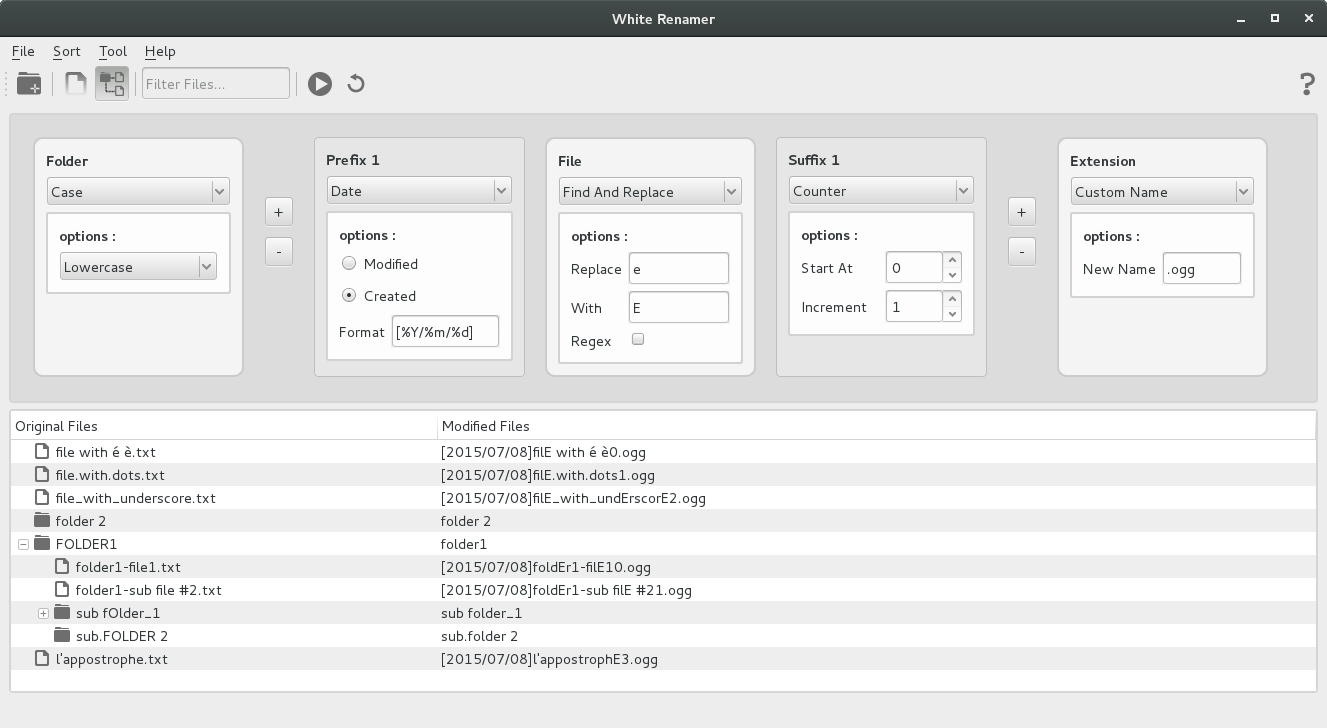
\includegraphics[width=1\textwidth]{MainLayout.png}
%\includegraphics[width=2cm]{logo.jpg}\\[-1em]
\vfill
\noindent
\color{white}
\makebox[0pt][l]{\rule{1.3\textwidth}{1pt}}
\par
\noindent
\textsf{\copyright{} Pierre Blanc}\hfill {\href{mailto:pierrecnalb@mailbox.org}{{\textsf{pierrecnalb@mailbox.org}}}}\\
\textsf{2015}
\thispagestyle{empty} % Remove page numbering on this page
\end{titlepage}
\restoregeometry % restores the geometry
\nopagecolor% Use this to restore the color pages to white
\renewcommand{\labelitemi}{$\bullet$}
%\tableofcontents
%%%%%%%%%%%%%%%%%%%%%%%%%
%%%%%%%%%%%%%%%%%%%%%%%%%
\section{Introduction}
White Renamer is a software that ease the pain of renaming multiple files and folders by doing it in batch. The user can choose many actions to perform on the selected directory. The following sections describes what those actions are, and how to use it.

\section{Description}
White Renamer has a simple UI containing two distinct parts : the top part displays boxes representing the structure of the files. \\
The first box : \emph{Folder} represents the changes made on the folders inside the selected directory.\\
The second box : \emph{File} represents the changes made on the files inside the selected directory.\\
The third box : \emph{Extension} represents the changes made on the extension of the files.\\
Some optional boxes can be inserted : \emph{Prefix} and \emph{Suffix} that give the possiblity to add prefix(es) or suffix(es) to the filename.\\

The bottom part displays a live preview of the changes made to the files/folders.


\section{Step by step}
\begin{enumerate}
        \item Select which directory you want to process.
        \item Select if you want to rename hidden directories.
        \item Select if you want to rename subfolders.
        \item Enter the desired pattern to rename only specific files.
        \item Sort by name(default), size or date in normal or reverse order.
        \item Add some prefixes and/or suffixes.
        \item Select the desired actions to perform on the folders, files and extensions.
        \item Press on Rename.
\end{enumerate}

\section{List of available actions}
The following actions are available :

\subsection*{Original Name}
(\emph{see figure \ref{OriginalName}})\\

No changes are made. The files or folders keep their original names.

\subsection*{Case}
(\emph{see figure \ref{Case}})\\

Three capitalization options are available :
\begin{itemize}
        \item \textbf{Titlecase} : gives the possiblity to uppercase the first letter of each words.
                \begin{itemize}
                        \item \emph{First Letter} : if checked, the first letter of the string will be capitalized. 
                        \item \emph{And After} : represents the characters after which the letter will go uppercase. 
                \end{itemize}
                E.g : if First Letter is checked and ``And After = \_'' the file \emph{my\_file} will become My\_File
        \item \textbf{Uppercase} : The whole string will be converted to uppercase.
        \item \textbf{Lowercase} : The whole string will be converted to lowercase.
\end{itemize}

\subsection*{Custom Name}
(\emph{see figure \ref{CustomName}})\\

\begin{itemize}
        \item \textbf{New Name} : changes the original name to the given new name.
\end{itemize}

\subsection*{Folder Name}
(\emph{see figure \ref{FolderName}})\\

Gives the name of the parent folder.

\subsection*{Find And Replace}
(\emph{see figure \ref{FindAndReplace}})\\

\begin{itemize}
        \item \textbf{Replace} : which characters should be replaced.
        \item \textbf{With} : with which characters the found token should be replaced.
        \item \textbf{Regex} : If checked, gives the ability to use regex. A list of commonly used regex is given below. For more information, please read the python re help page.
                \begingroup
                \fontsize{8pt}{8pt}\selectfont
\begin{verbatim}
The special characters are:
       "."      Matches any character except a newline.
       "^"      Matches the start of the string.
       "$"      Matches the end of the string or just before the newline at
                the end of the string.
       "*"      Matches 0 or more (greedy) repetitions of the preceding RE.
                Greedy means that it will match as many repetitions as possible.
       "+"      Matches 1 or more (greedy) repetitions of the preceding RE.
       "?"      Matches 0 or 1 (greedy) of the preceding RE.
       *?,+?,?? Non-greedy versions of the previous three special characters.
       {m,n}    Matches from m to n repetitions of the preceding RE.
       {m,n}?   Non-greedy version of the above.
       "\\"     Either escapes special characters or signals a special sequence.
       []       Indicates a set of characters.
                A "^" as the first character indicates a complementing set.
       "|"      A|B, creates an RE that will match either A or B.
       (...)    Matches the RE inside the parentheses.
                The contents can be retrieved or matched later in the string.
       (?aiLmsux) Set the A, I, L, M, S, U, or X flag for the RE (see below).
       (?:...)  Non-grouping version of regular parentheses.
       (?P<name>...) The substring matched by the group is accessible by name.
       (?P=name)     Matches the text matched earlier by the group named name.
       (?#...)  A comment; ignored.
       (?=...)  Matches if ... matches next, but doesn't consume the string.
       (?!...)  Matches if ... doesn't match next.
       (?<=...) Matches if preceded by ... (must be fixed length).
       (?<!...) Matches if not preceded by ... (must be fixed length).
       (?(id/name)yes|no) Matches yes pattern if the group with id/name matched,
                          the (optional) no pattern otherwise.

   
The special sequences consist of "\\" and a character from the list
below.  If the ordinary character is not on the list, then the
resulting RE will match the second character.
    \number  Matches the contents of the group of the same number.
    \A       Matches only at the start of the string.
    \Z       Matches only at the end of the string.
    \b       Matches the empty string, but only at the start or end of a word.
    \B       Matches the empty string, but not at the start or end of a word.
    \d       Matches any decimal digit; equivalent to the set [0-9] in
             bytes patterns or string patterns with the ASCII flag.
             In string patterns without the ASCII flag, it will match the whole
             range of Unicode digits.
    \D       Matches any non-digit character; equivalent to [^\d].
    \s       Matches any whitespace character; equivalent to [ \t\n\r\f\v] in
             bytes patterns or string patterns with the ASCII flag.
             In string patterns without the ASCII flag, it will match the whole
             range of Unicode whitespace characters.
    \S       Matches any non-whitespace character; equivalent to [^\s].
    \w       Matches any alphanumeric character; equivalent to [a-zA-Z0-9_]
             in bytes patterns or string patterns with the ASCII flag.
             In string patterns without the ASCII flag, it will match the
             range of Unicode alphanumeric characters (letters plus digits
             plus underscore).
             With LOCALE, it will match the set [0-9_] plus characters defined
             as letters for the current locale.
    \W       Matches the complement of \w.
    \\       Matches a literal backslash.


\end{verbatim}
         \endgroup
\end{itemize}

\subsection*{Insert Characters}
(\emph{see figure \ref{Insert}})\\

\begin{itemize}
        \item \textbf{Insert} : what characters should be inserted.
        \item \textbf{At Position} : position, in the original name, of the characters to be inserted. 0 represents the beginning of the string.
\end{itemize}

\subsection*{Delete Characters}
(\emph{see figure \ref{Delete}})\\

\begin{itemize}
        \item \textbf{From} : starting position of the characters to remove.
        \item \textbf{To} : ending position of the characters to remove.
\end{itemize}

\subsection*{Counter}
(\emph{see figure \ref{Counter}})\\

\begin{itemize}
        \item \textbf{Start At} : starting number of the counter. 
        \item \textbf{Increment} : increment number of the counter.
\end{itemize}

\subsection*{Date}
(\emph{see figure \ref{Date}})\\

\begin{itemize}
        \item \textbf{Modified} : date of the last modification.
        \item \textbf{Created} : date of the creation.
        \item \textbf{Format} : date format specification. Commonly used formats are :
                \begingroup
                \fontsize{8pt}{8pt}\selectfont
\begin{verbatim} 
%Y  Year with century as a decimal number.
%m  Month as a decimal number [01,12].
%d  Day of the month as a decimal number [01,31].
%H  Hour (24-hour clock) as a decimal number [00,23].
%M  Minute as a decimal number [00,.8].
%S  Second as a decimal number [00,61].
%z  Time zone offset from UTC.
%a  Locale's abbreviated weekday name.
%A  Locale's full weekday name.
%b  Locale's abbreviated month name.
%B  Locale's full month name.
%c  Locale's appropriate date and time representation.
%I  Hour (12-hour clock) as a decimal number [01,12].
%p  Locale's equivalent of either AM or PM.
\end{verbatim}
        \endgroup
\end{itemize}

\section{Examples}

\begin{figure}[!ht]
        \centering
        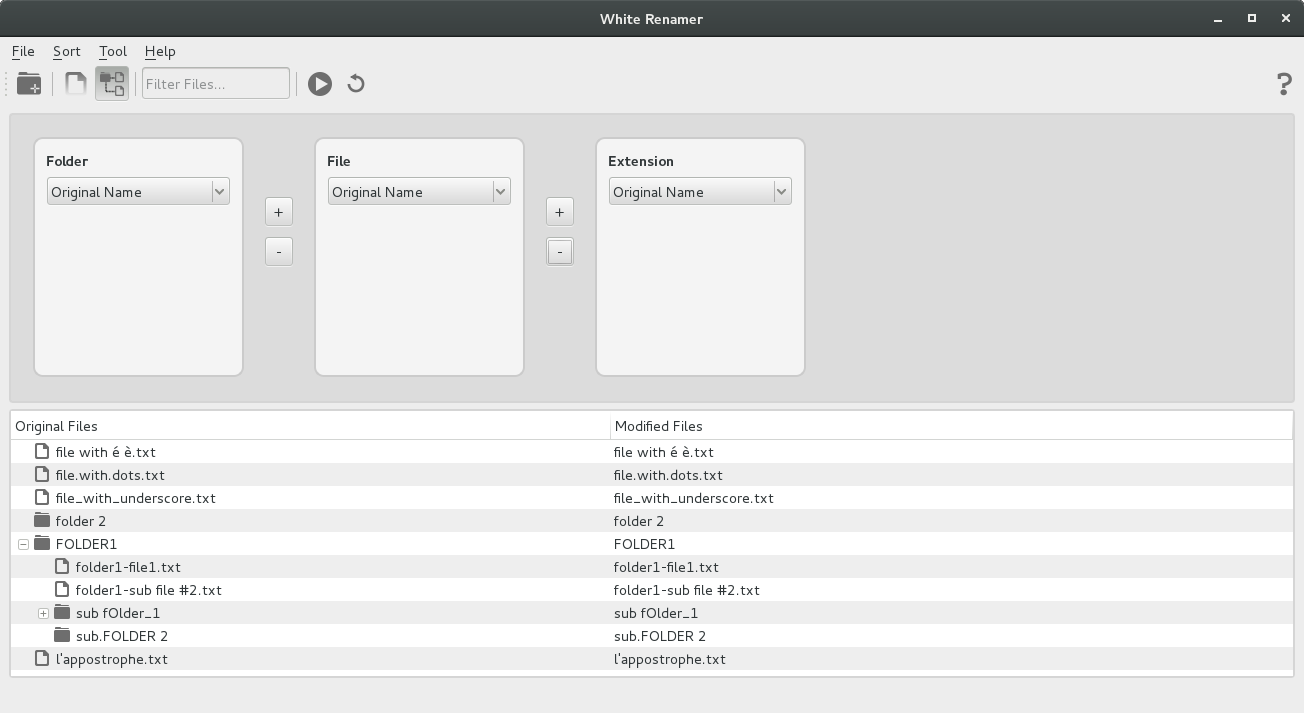
\includegraphics[width=\textwidth]{OriginalName.png}
        \caption{Original Name option example.}
        \label{OriginalName}
\end{figure}
\begin{figure}[!ht]
        \centering
        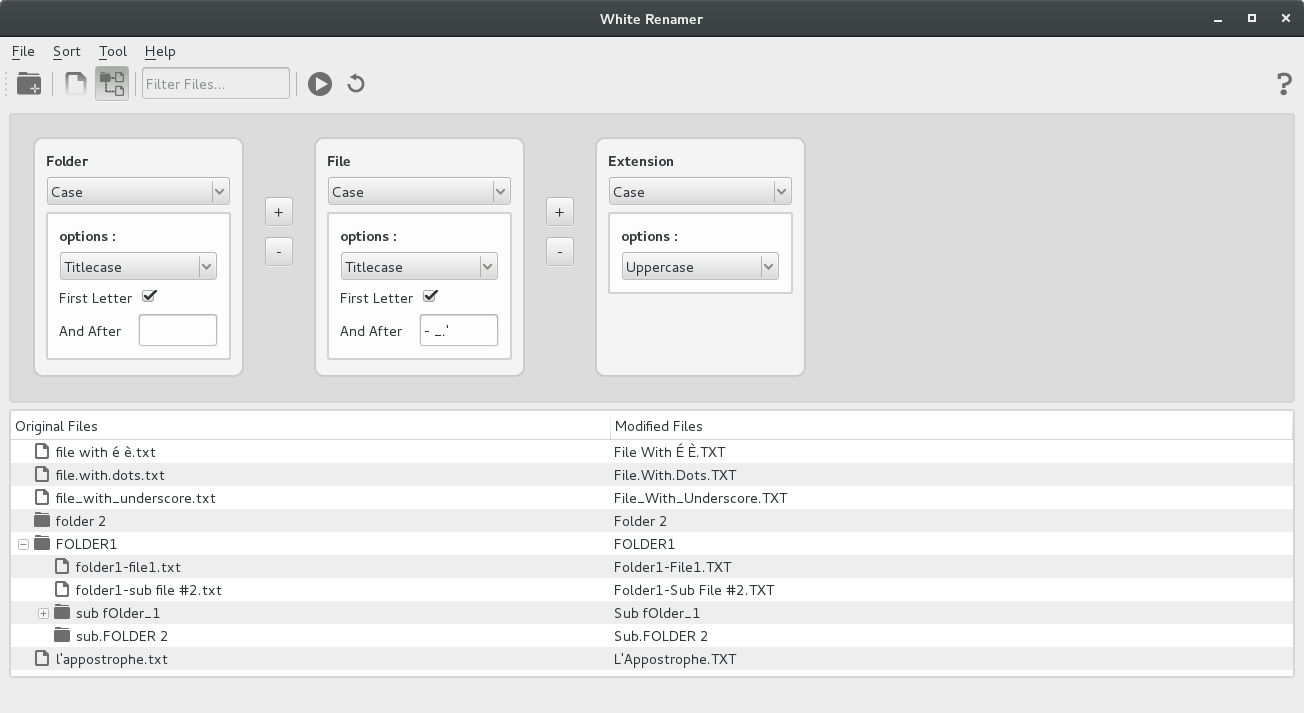
\includegraphics[width=\textwidth]{Case.png}
        \caption{Case option example.}
        \label{Case}
\end{figure}
\begin{figure}[!ht]
        \centering
        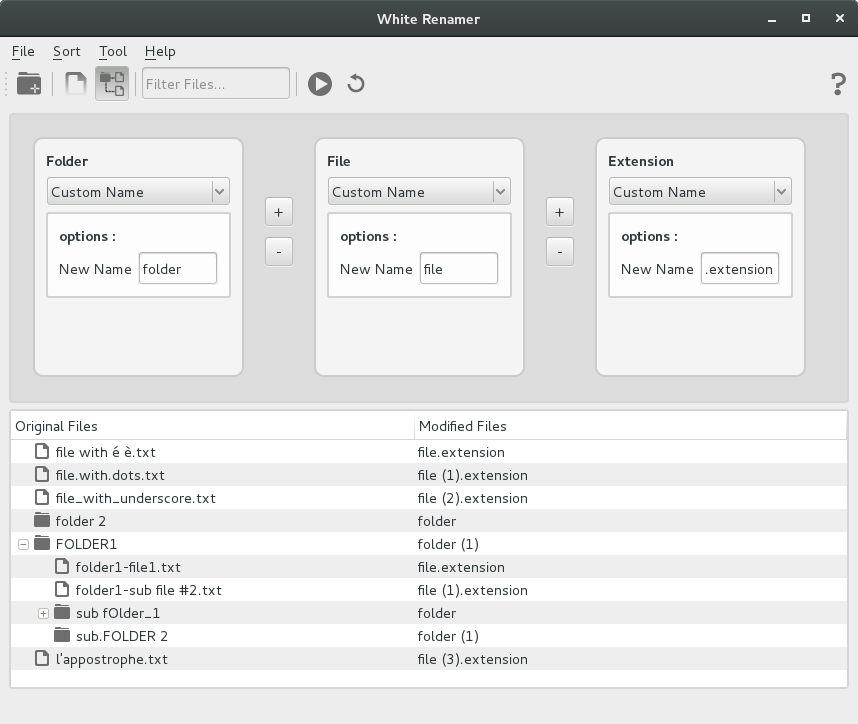
\includegraphics[width=\textwidth]{CustomName.png}
        \caption{Custom Name option example.}
        \label{CustomName}
\end{figure}
\begin{figure}[!ht]
        \centering
        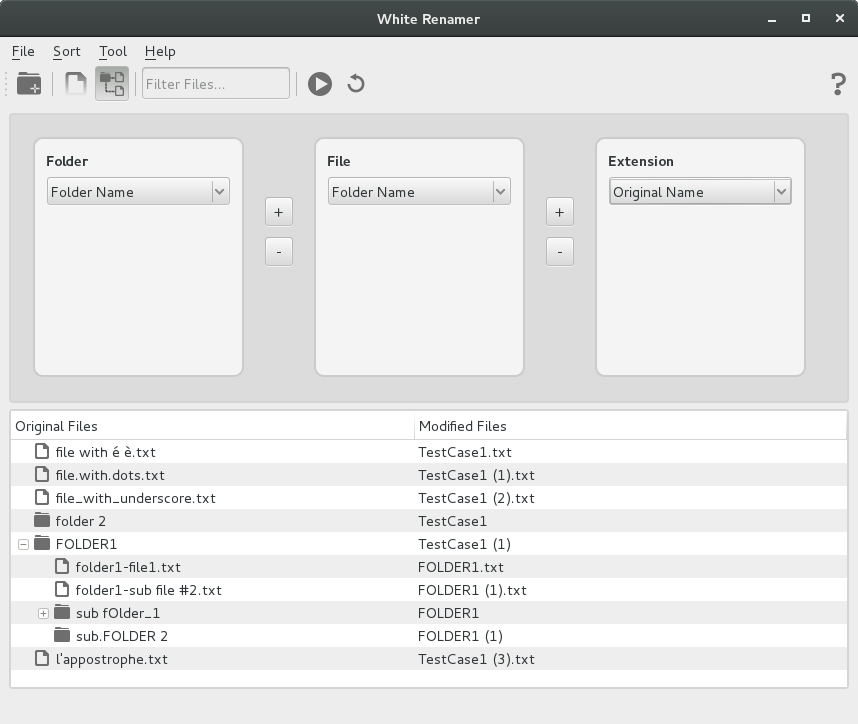
\includegraphics[width=\textwidth]{FolderName.png}
        \caption{Folder Name option example.}
        \label{FolderName}
\end{figure}
\begin{figure}[!ht]
        \centering
        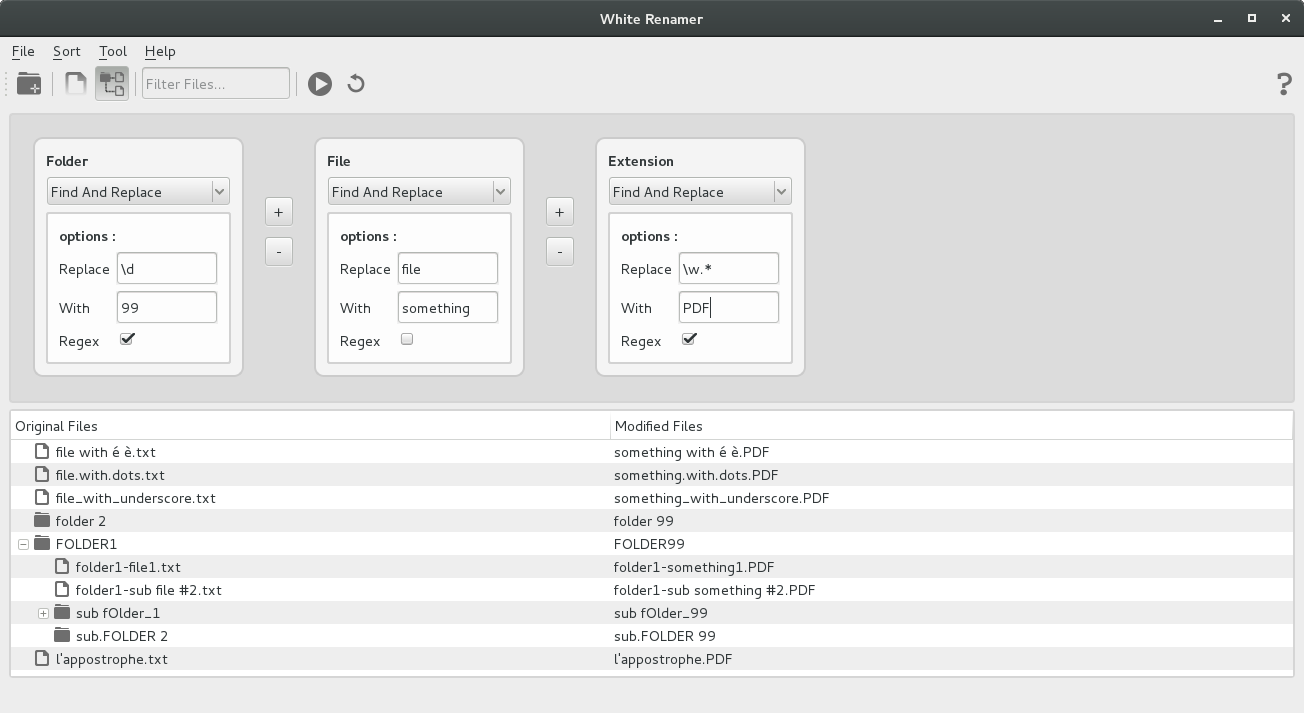
\includegraphics[width=\textwidth]{FindAndReplace.png}
        \caption{Find And Replace option example.}
        \label{FindAndReplace}
\end{figure}
\begin{figure}[!ht]
        \centering
        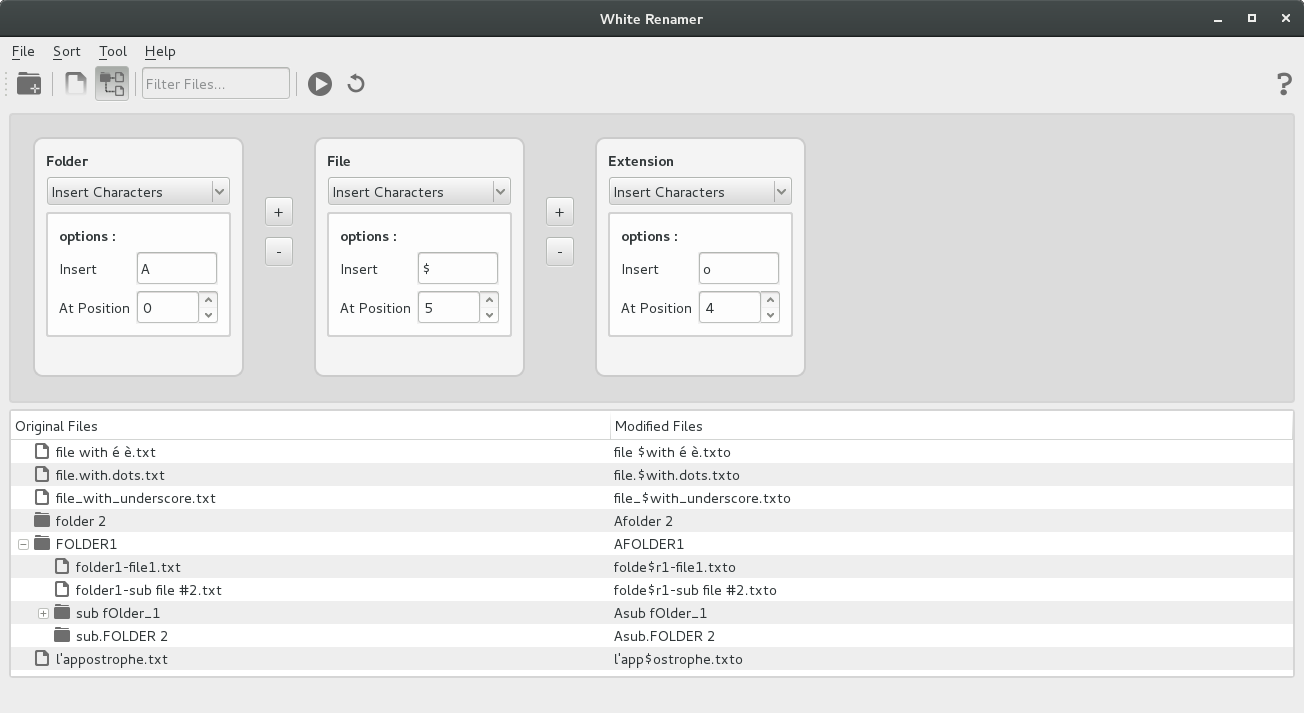
\includegraphics[width=\textwidth]{Insert.png}
        \caption{Insert Characters option example.}
        \label{Insert}
\end{figure}
\begin{figure}[!ht]
        \centering
        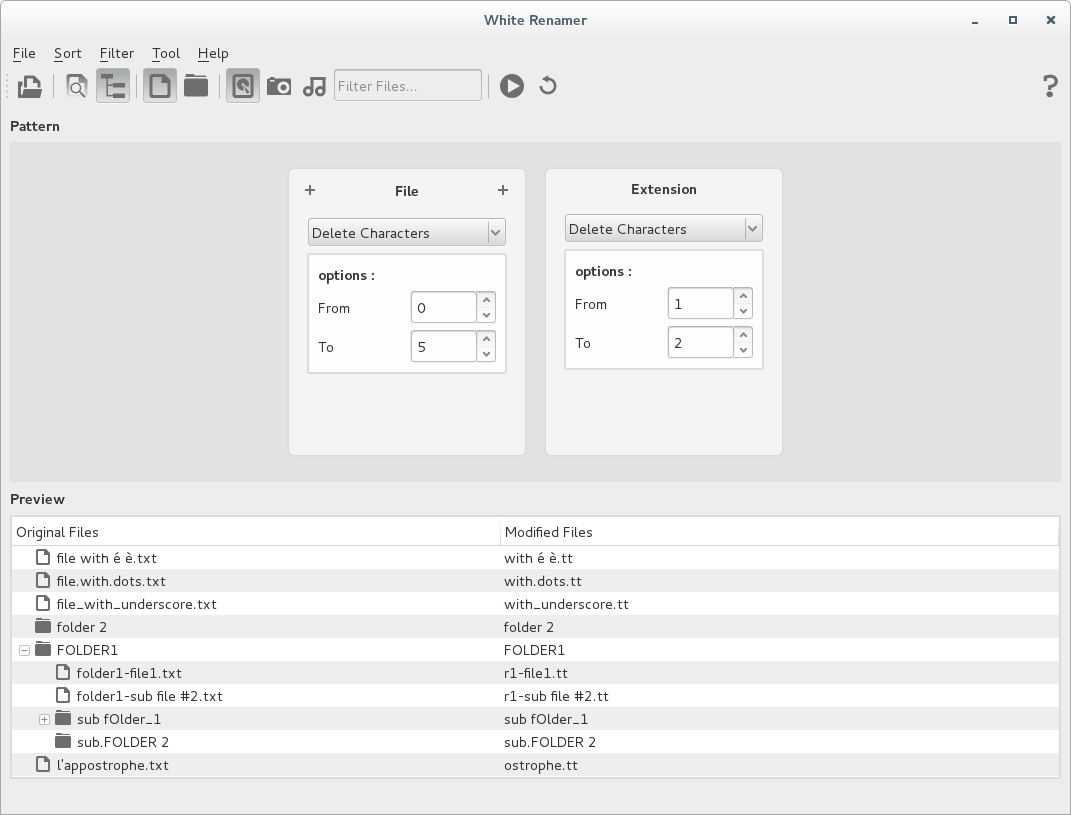
\includegraphics[width=\textwidth]{Delete.png}
        \caption{Delete Characters option example.}
        \label{Delete}
\end{figure}
\begin{figure}[!ht]
        \centering
        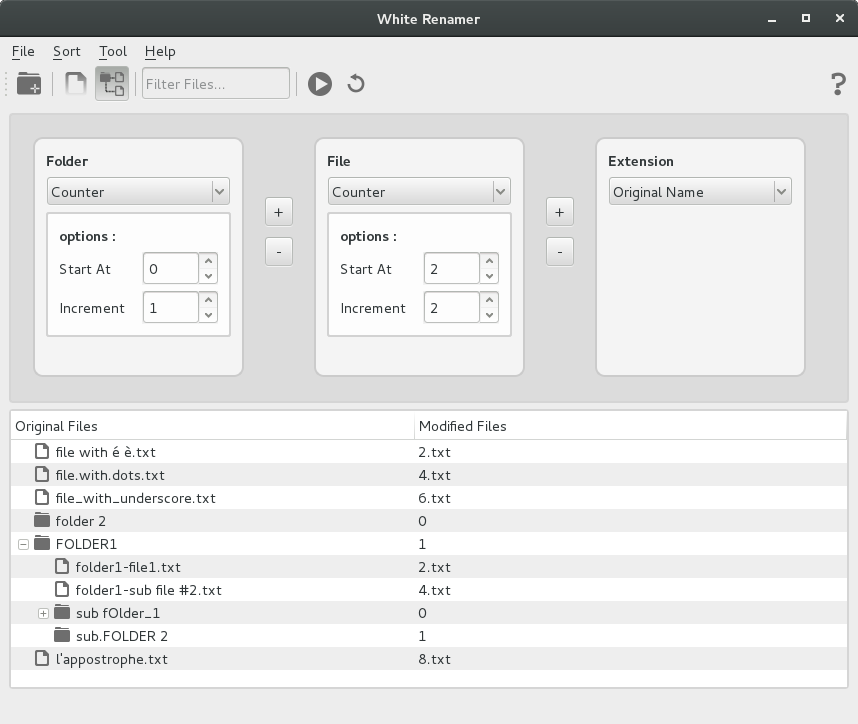
\includegraphics[width=\textwidth]{Counter.png}
        \caption{Counter option example.}
        \label{Counter}
\end{figure}
\begin{figure}[!ht]
        \centering
        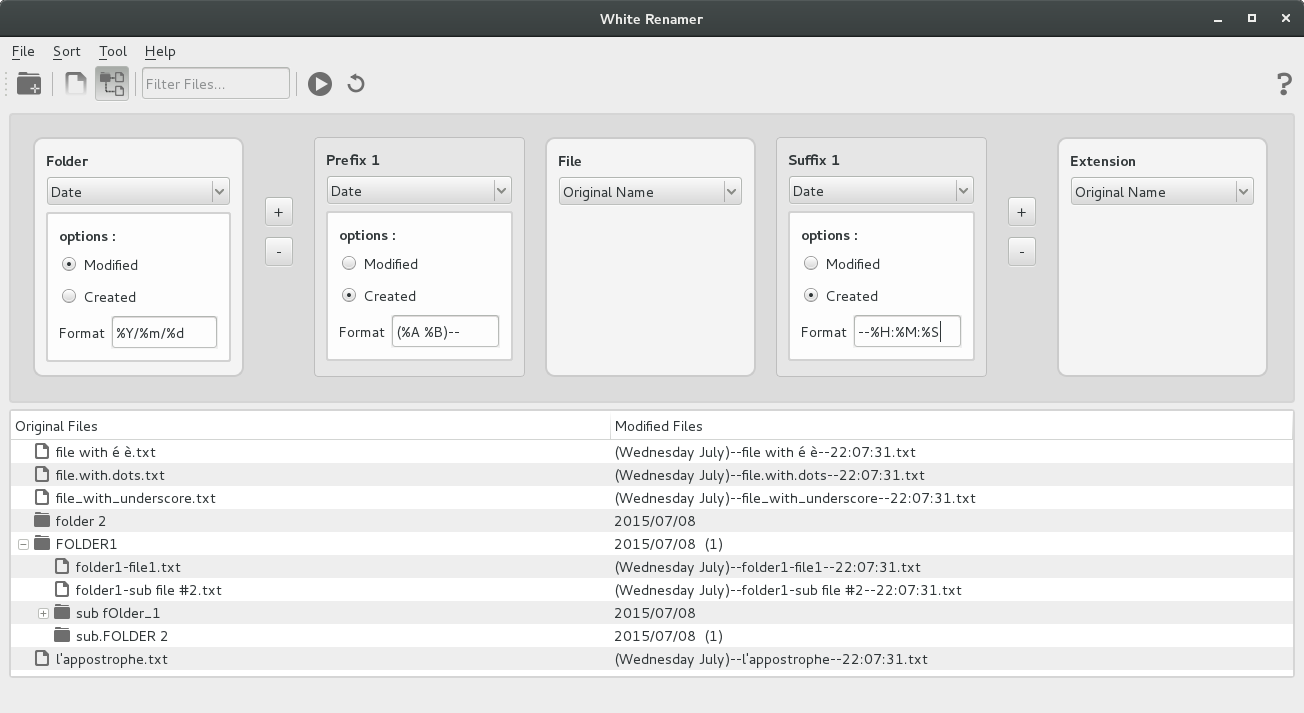
\includegraphics[width=\textwidth]{Date.png}
        \caption{Date option example.}
        \label{Date}
\end{figure}

\end{document}
